\documentclass{article}

\usepackage{Sweave}
\begin{document}
\Sconcordance{concordance:p3.tex:/home/oski/stat243/problem3/p3.Rnw:%
1 2 1 1 0 6 1 1 2 5 0 2 2 1 0 1 1 3 0 1 2 1 1}

\noindent \textbf{The result of your solution to Problem 3 should look like this page}


The height of the water level in Lake Huron fluctuates over time. Here I 'analyze' the variation using R. I show a histogram of the lake levels for the period 1875 to 1972.

\begin{Schunk}
\begin{Sinput}
> hist(LakeHuron)
\end{Sinput}
\end{Schunk}
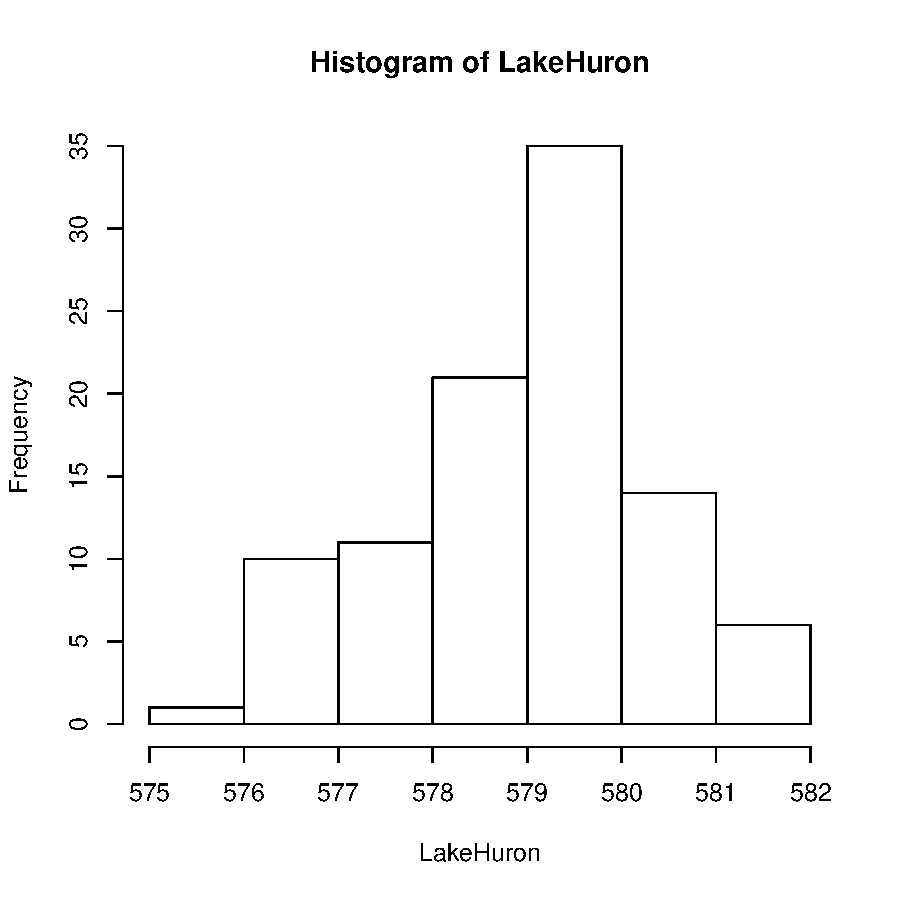
\includegraphics{p3-001}

\begin{Schunk}
\begin{Sinput}
> lowHi <- c(which.min(LakeHuron), which.max(LakeHuron))
> yearExtrema <- attributes(LakeHuron)$tsp[1]-1 + lowHi
\end{Sinput}
\end{Schunk}

\end{document}
